\documentclass[11pt]{article}

\usepackage{blindtext}
\usepackage[pdftex]{graphicx}
\usepackage{fancyhdr}
\usepackage[margin=1in]{geometry}
\usepackage[hang]{footmisc}
\usepackage{lipsum}
 \usepackage[flushleft]{threeparttable}
 \usepackage{tabularx} 
\usepackage{apacite}
\usepackage{float}
\usepackage{caption}
\usepackage{subcaption}
%\pagestyle{headings}
%\fancyhf{}
%\rhead{djfklas}
%\lhead{dkjfalj}
%\rfoot{ Page \thepage}
\usepackage{breqn}
\usepackage{titlesec}
\usepackage[labelfont={bf}]{caption}
%\usepackage{hyperref}
\usepackage{setspace}
\interfootnotelinepenalty=10000
\usepackage{arydshln}
\usepackage{rotating}
\doublespacing
\newcolumntype{Y}{>{\centering\arraybackslash}X}

\def\sym#1{\ifmmode^{#1}\else\(^{#1}\)\fi}

\rfoot{ Page \thepage}
%
%\titleformat{\section}
%  {}{\thesection}{1em}{\textbf}
%  
% \titleformat{\subsection}
%  {\scshape}{\thesubsection}{1em}{\textbf}
%  
%  
%  \titleformat{\subsubsection}
%  {\scshape}{\thesubsubsection}{1em}{\textbf}
  
\newcommand\blfootnote[1]{%
  \begingroup
  \renewcommand\thefootnote{}\footnote{#1}%
  \addtocounter{footnote}{-1}%
  \endgroup
}

\title{ Effects of a Minimum Wage Increase on Restaurants: \\ Price Pass Through and Beyond}
\author{Chelsea Crain \footnote{Department of Economics, University of Iowa, Iowa City, IA, \textit{Email: }chelsea-crain@uiowa.edu} }

\begin{document}

\maketitle

\begin{abstract}
In this paper, I analyze the effects of a minimum wage increase on restaurants. Using a novel dataset comprised of menu item information from thousands of east coast restaurants across six states from Yelp.com and Grubhub.com, I isolate the effects of varying levels of minimum wage increases. I find that prices rise in response to a minimum wage increase as predicted by the competitive model of labor markets. I furthermore find that these price pass through effects are stronger for certain types of menu items and for restaurants who have low levels of consumer ratings prior to the minimum wage hike. I also find that increases in minimum wage increase the level of customer perceived quality of restaurants.

\end{abstract}



\section{Introduction}
%The primary aspect of policy change impact I will analyze is the price pass-through to consumers. 
A great deal of research has been done on the effects of minimum wage increases on prices, but the unique nature of the dataset and policies that I use in this paper allow for additional minimum wage related questions to be answered. The restaurant industry is the primary focus of this minimum wage study due to the high employment rates of minimum wage workers in the industry. I take advantage of a natural experimental setting across six contiguous states on the East coast, where all states increased their respective minimum wages (though by differing magnitudes) on the first of 2017. The primary dataset used for this study is a novel dataset comprised of restaurant and menu information collected from Yelp.com, with multiple waves of observations both before the policy implementation as well as after. The data allow for analysis at the restaurant level as well as the item level. In addition to price pass-through, I analyze how customer-perceived quality of the restaurant is affected by increases in minimum wage using Yelp stars. The price pass through effects are also analyzed using a second source of restaurant and item level data, Grubhub.com.

This study adds to the literature by providing a unique and detailed dataset that allows for rigorous testing of the price pass through to consumers at the restaurant and item level, additionally providing analysis of relevant, non-price impacts of a minimum wage increase. I find that, on average, a 10 percent increase in the minimum wage leads to a 0.3 percent increase in prices within the first month following a minimum wage increase. The price pass through is highest for restaurants that begin with a below average Yelp rating and for non-chain restaurants. Price pass through is higher for certain types of menu items, such as sides and sandwiches. Lastly, I find that a 10 percent increase in minimum wage increases the consumer Yelp rating of restaurants by 0.4 percent on average.

\section{Motivation}

Since the publication of Card and Kruger's well known study about the effects of minimum wage changes on the fast food industry in 1994\nocite{card1994minimum}, the literature on minimum wage effects has become widespread. Card and Kruger found a small positive effect on employment and no effect on prices after an increase in the minimum wage. These findings contradicted the textbook model of competitive labor markets, which predicts an increase in output prices and a decrease in employment. In response to this paper, many studies were published analyzing the existence of monopsony power in the labor market \cite{manning1995we, rebitzer1995consequences, burdett1998wage, bhaskar1999minimum} to explain the small employment effects seen in the data. However, in a survey of the literature by Neumark and Wascher (2006)\nocite{neumark2006minimum'}, it is concluded that the most rigorous and reliable studies have found significant price increases but small employment decreases. As Aaronson, French and MacDonald conclude in their 2008 publication\nocite{aaronson2008minimum}, the presence of significant increases in price in response to minimum wage increases is evidence against the prevalence of monopsony power in the labor market. 

Although there is evidence against the prevalence of monopsony power in the labor market, there is still a discrepancy between what is predicted in the models and what is seen in the data.  Under labor market models of competition, monopsonistic competition, and even efficiency wages, a relatively large increase in price should be accompanied by a relatively large decrease in employment \cite{aaronson2008minimum}. Thus the question begs, in what other ways are restaurants offsetting the increases in labor costs? Some suggestions that have been made in the literature include changes in non-wage compensation and the ``hungry teenager hypothesis''\cite{kennan1995elusive}. This hypothesis suggests that the increase in income seen by minimum wage workers causes them to purchase more minimum wage products, thus offsetting some of the dis-employment effects. However, MacCurdy and O'Brien-Strain (2000) estimate that this could account for only 10 to 30 percent of the employment loss\nocite{macurdy2000increasing}. 

One way that restaurants could absorb the increase in labor costs, other than by increasing price or decreasing employment, is to decrease quality. Unlike data used in previous studies, the unique dataset used in this paper allows for analysis of changes in customer-perceived quality. Two other ways that restaurants may cut corners to make up for increased labor costs is to decrease the number of items offered on the menu, or to decrease hours of operation. Most previous studies have focused on a few menu items, or a few bundles of items and are therefore not able to analyze changes within the full menus. In addition to full menu analysis, the dataset used in the present study also provides the ability to look at the type of menu item, such as an appetizer versus a main dish, which is unique to the literature. 


%From a policy perspective, one of the proposed negative effects of a minimum wage increase is the inability of restaurants close to the border of the city or state to account for these increased input costs without loosing business. It is thought that restaurants facing minimum wage increases close to a border where competitors on the opposite side of the border are not facing an increase in labor costs may have to keep prices artificially low in order to compete. These effects are referred to as border effects. To think of this effect in more detail, imagine a simplified world in which there are two restaurants  on opposite sides of a state line competing in a market, where one state is increasing the minimum wage and the other is not. The business who is facing no increase in minimum wage knows about the increase in labor costs to their competitor, and thus as Chicu, Vickers, and Ziebarth (2012) find, the increase in the competitor's cost may have a positive effect on the restaurant's own price. This effect may also hold true in the opposite direction, where a restaurant facing a minimum wage increase that is close to a border where competitors are facing no increase may have a negative effect on the price increase. If there are border effects, these effects would be predicted to dissipate as the distance from the restaurant to the border increases. 

%The existence of border effects have different implications depending on the side of the border in which they exist. If there are significant border effects on the side of the border where there is a lower minimum wage increase, this would imply that workers and consumers are hurt by the minimum wage increase of the other state. Workers and consumers would be hurt since they are seeing an increase in prices but none of the employees are receiving a higher wage. If there are significant border effects on the side of the border where there is a higher minimum wage increase, this would imply that businesses are hurt by the minimum wage increase because they are forced to keep prices artificially low in order to compete with other businesses.

%Therefore, for the purposes of this paper it will be assumed that the labor market is competitive and that there is monopolistic competition in the output market following Dixit-Stiglitz (19977)\nocite{dixit1977monopolistic}.





\section{Minimum Wage Laws}

Across the United States there has been a large push from workers to increase the minimum wage, commonly referred to as the ``Fight for \$15'' \cite{ff15}. In response, some cities and states have taken matters into their own hands and increased the minimum wage above the current state minimum wage, which in some cases, was already above the federal minimum wage of \$7.25. On January 1, 2017, six contiguous states on the east coast increased their minimum wage at differing magnitudes, with a variety of different levels of increase within the state of New York. Table 1 reports the increases in minimum wage in these areas, which range from 0 to 22\%\footnote{The last three columns of Table 1 report any changes in the tipped minimum wage. In the leisure and hospitality industry as a whole, the Bureau of Labor Statistics report that tipped workers constitute only 12.5\% of the labor force. Since the tipped minimum wages are well below the regular minimum wages, labor costs from tipped minimum wage workers are even smaller.}

 In April of 2016, New York became the second state, after California, to pass a law that would incrementally raise the minimum wage for all workers to \$15 \cite{nybill}. In 2015, prior to this \$15 minimum wage law for all workers, New York passed a minimum wage law only applicable to fast food restaurants, increasing the minimum wage each year for fast food workers with a steeper increase for workers in down town New York City \cite{nyff}. The first two rows of Table 1 report the 2016 and 2017 minimum wages for fast food workers in both NYC and in the rest of the state. In the more recent 2016 New York minimum wage law, which applies to non-fast food workers, the degree of the minimum wage increase is based on the type and location of the establishment \cite{nybill}. Groups 3 and 4 report minimum wage changes for non-fast food restaurants in downtown NYC, with the magnitude of the increase dependent on if the restaurant is large or small, where large is defined as employing more than 10 workers. Group 5 includes non-fast food restaurants of all sizes in the three contiguous counties outside of NYC: Nassau, Suffolk, and Westchester. Group 6 includes non-fast food restaurants of all sizes elsewhere in the state of New York. 
 
The five contiguous states to New York have varying changes in their own state-wide minimum wage laws which all went into effect January 1, 2017.  In July of 2014, Connecticut passed a law that would increase the minimum wage for all workers in small increments each year until 2017, where it would reach \$10.10 \cite{ctbill}. In 2016, New Jersey proposed a minimum wage law similar to that of New York that would put workers on the track to a \$15 minimum wage. The bill passed through the house and the senate, but in September of 2016, governor of New Jersey Chris Christie vetoed the bill, stating ``...[this bill] fails to consider the capacity of businesses, especially small businesses, to absorb the substantially increased labor costs it will impose''\cite{njveto}. Thus in 2017 New Jersey increased the state minimum wage by only 0.72\%, a yearly adjustment for inflation \cite{njbill}. Massachusetts passed a bill in 2014 that increased the minimum wage by \$1 a year starting at the beginning of 2015. The state will see the final increase relating to this bill on January 1 of 2017 \cite{mabill}. A large group of workers in Pennsylvania pushed for an increase in the minimum wage, but the group had no luck in persuading the politicians in their state. Workers in Pennsylvania saw no increase in the minimum wage at the beginning of 2017 \cite{panobill}. Similar to the minimum wage law in Connecticut, Vermont passed a minimum wage law in 2013 that increased the minimum wage for the state each year from 2014-2018, providing workers with a 4.2\% increase in minimum wage at the beginning of 2017 \cite{vtbill}. Together, the minimum wage laws of these six states provide a unique natural experimental setting in which to analyze the effects of a minimum wage increase. 




\section{Data}

Three primary datasets will be used in this analysis. The first, and most extensive,  is a panel dataset comprised of restaurant and menu information from Yelp.com. The second is a supplementary panel dataset also comprised of restaurant and menu information from Grubhub.com.  The third is a dataset providing detailed restaurant business information from ReferenceUSA. These datasets will be utilized to determine the magnitude of price pass through to consumers, how this pass-through varies by restaurant and item specific characteristics, and how the minimum wage affected customer percieved quality.

\subsection{Yelp}

Yelp.com is a website in which consumers can find restaurant information including customer reviews, hours of operation, price range, and full menus. Yelp was founded in 2004, and currently has an average of 72 million monthly visitors with over 115 million reviews written \cite{yelpstat}. Although it is not possible to verify that every restaurant in the areas of interest has information on Yelp, I will later compare the Yelp dataset to the ReferenceUSA dataset to determine the representativeness of the restaurants in my sample. The first wave of Yelp data collection was in April 2016, the second wave in July 2016, the third wave in October 2016, and the fourth in January 2017. Future waves of data collection will occur in February, March, and April 2017.

To collect a geographically representative sample, a list of areas of interest was compiled spanning all six states and focusing more heavily on larger cities. Using a webscrape for each area in the list, all Yelp restaurant home pages and menu pages were downloaded. The Yelp homepage of each restaurant contains information about the restaurant including address, phone number, Yelp star rating, price range, food category and hours of operation. Approximately one third of these restaurants provide a full menu on their Yelp page.\footnote{Some restaurants provide an external link to a menu, but since these menus are not formatted uniformly, the menu information cannot be correctly parsed and thus for the sake of this dataset these restaurants fall into the same category of those restaurants who do not provide an online menu. In a similar study using online menus, Allegrotto (2016) also found that on average about one third of restaurants posted full online menus\nocite{allegretto2016local}.} These menus provide item category and price information that is parsed into a usable dataset along with the other restaurant characteristics. Figure 1 shows the geographical distribution of the restaurants in the sample.

One concern with using Yelp data is the reliability and frequency with which the information for a restaurant is updated, as Yelp menus may be updated at the restaurant owner or manager's discretion. As a way to deal with this reliability issue, I take advantage of a food delivery service that is powered by Yelp called Eat24. This service provides customers the ability to order food directly from the restaurant's Yelp menu page for delivery or pickup. The use of this service ensures that the menu items and prices are up to date since customers are ordering directly from the provided menu information. Each restaurant in the dataset has an indicator for whether or not the business utilizes the Eat24 service. 

Although the number of stars that a restaurant has earned is determined by self-selected reviewers, the number of Yelp stars has been found to be a reliable predictor of actual quality as well as an important determinant of profit for restaurants. In a study comparing Yelp star ratings of hospitals to an industry standard assessment of quality, Bardach et. al (2014) found that Yelp stars were significantly related to patient care and health outcomes. Luca (2011) used a regression-discontinuity design to analyze the impact of a change in the  rounded Yelp star rating on restaurants, and found that a one-star increase in the Yelp rating led to a 5-9\% increase in revenue. Another concern of using Yelp stars as a point of analysis regards restaurants writing fake reviews-- good reviews of themselves and bad reviews of competitors. Yelp uses a proprietary algorithm in an attempt to filter out fake reviews which are in turn not included in the Yelp star rating. Although some fake reviews may still exist, I will assume for the analysis that the reviews are an unbiased source to measure overall consumer perceived quality of a restaurant. 

The rounded star rating that customers see prominently displayed on each restaurant's hoempage is the monthly average of all Yelp reviews rounded to the nearest half star.\footnote{If a restaurant has less than 10 reviews within a month, then the most recent reviews are added until the sample size reaches 10.} There is significant variation in the exact Yelp star rating per month for restaurants, an indication that Yelp users are active in reporting the currennt quality of the establishments. Over 70 percent of restaurants see a change in exact star rating between any given observation period, and the average change given an increase (decrease) is 0.37 (0.39) stars.


\subsection{GrubHub} 

Founded in 2004, Grubhub.com is the largest online food ordering company in the U.S., providing its 7.7 million customers in over 1,100 cities accesss to delivery at over 45,000 locations \cite{grubstat}. Menu information for all GrubHub restaurants in the areas of interest was collected using a webscrape in December 2016 and January 2017. Further waves of data collection will occur in February, March, and April of 2017. Although there are fewer restaurants on Grubhub than there are on Yelp, the GrubHub menu prices, which are necessarily up to date, provide an idea to what extent the Yelp data is generalizable. Grubhub also allows customers to rate the restaurants, but there are significantly fewer reviews given on Grubhub than there are on Yelp. Grubhub restaurants are also primarily in the more highly populated areas and therefore sample sizes for the smaller cities are much lower in the Grubhub data.


\subsection{ReferenceUSA}

Since the magnitudes of the minimum wage increases are dependent on the type of establishment for those business in New York, I use ReferenceUSA, an Infogroup company that provides accurate and complete business data. I collect the data for all businesses that are categorized under the North American Industry Classification System (NAICS) as a restaurant. I gather data from all restaurants in the areas of interest in order to use this dataset as the population. As a measure of the validity of the decision to use ReferenceUSA as the population I look to the New York City Department of Health and Mental Hygiene. The Department of Health and Mental Hygiene is required to keep a list of all business that perform any kind of food service, of which there are 26,047 listed. This list, however, contains businesses such as country clubs, banks, and concession stands, which would not be in the ReferenceUSA dataset by construction. In the ReferenceUSA dataset there are 24,228 restaurants. Therefore, although not a perfect match, I assume for the rest of the analysis that the ReferenceUSA dataset is representative of the true population.



\subsection{Data Construction and  Definitions}

The restaurant characteristic definitions are key to understanding the effects of the minimum wage increases. A limited service (LS) restaurant is one in which customers generally order and pay for items before eating. A full service (FS) restaurant is defined as an establishment where customers sit down to eat, and where the food is served directly to the customers' table, and the customers pays after eating. The ReferenceUSA data contains the NAICS codes from which I can determine the LS or FS status of a restaurant. For this study, a chain restaurant is defined as having a franchise status in the ReferenceUSA dataset. A fast food (FF) establishment is defined as a restaurant that is both LS and a chain, the definition used in the New York minimum wage laws. A large restaurant will be defined as one employing more than 10 workers, which once again follows the definition used by the state of New York.

Table 2 shows the sample construction of the dataset, where ReferenceUSA is used as the population. The proportion of LS and chain restaurants for both datatsets decreases at each level of sample construction. From this table it can be concluded that LS and chain restaurants are slightly less likely to be on Yelp, and significantly less likely to have a menu posted on Yelp that contains prices. This is consistent with Allegrotto and Reich (2015) who found that many chains do not post menus with store specific prices online.\nocite{allegretto2016local}\footnote{For example, McDonald's only posts menu prices on electronic menu boards inside each establishment.} There is also less motivation for chain restaurants to have complete and updated Yelp profiles, as they are not as strongly effected by the quality of their Yelp presence \cite{luca2011reviews}. From a political perspective, one of the biggest concerns of a minimum wage increase is the welfare of the small businesses. This dataset, although somewhat under-representative of the chain restaurants, has the ability to provide more insight into the effects of a minimum wage increase on these small businesses. %Table 3 reports sample sizes across minimum wage  groups.

Table 3 reports extensive descriptive statistics of restaurant characteristics by minimum wage group and data source. The reported statistics are from the data collection wave in October 2016. In order to create a balanced panel, I use only restaurants that are in each wave of data collection and only those menu items that are consistently on the menu.\footnote{Some restaurants may decide to post their own, external menu on Yelp and so could be in one wave of data collection but not another.} Since I match menu items across time by name, I cannot distinguish between a change in item name and removal of an item. Average number of items and average price per item per restaurant are both calculated using all menu items, regardless of which items are consistent over time. Therefore average price and total number of items may provide different information than item specific changes. There are differences across minimum wage groups and across the data source from which the data were collected. The restaurants within in a minimum wage group are not necessarily the same restaurants across Yelp and Grubhub. %There are however, 1,395 restaurants that are in both the Yelp and Grubhub datasets.
Because of the small sample sizes and unique characteristics of the fastfood restaurants in the dataset, all fast food restaurants will be excluded from the analysis. This removes 68 restaurants from the sample, 31 of which are from New York.

%Table 4 provides summary statistics regarding price changes in Yelp menu items. ( These are all pre-min wage change. Need to add post-min wage change and discuss differences and similarities)




%To analyze border effects, multiple definitions in the data need to be made. Take any restaurant in the dataset for which there is price information available and which has been matched to the ReferenceUSA database. To find if there are any border effects in the positive direction, I first find all restaurants in the population that face a higher minimum wage increase than the sample restaurant. Out of those restaurants, I define a competitor to be a restaurant which has the same LS and chain characteristics of the sample restaurant. Finally, out of the group of restaurants in the population that are defined as competitors and who face a higher minimum wage than the sample restaurant, I use Google maps API to find the shortest driving time to a competitor.\footnote{I restrict the distance to be within 30 miles, as I am only interested in effects for establishments relatively close to a state or county border.} This driving time is the value that will be used as the ``distance to the nearest competitor facing a higher minimum wage increase.'' The same methods are used to find ``distance to the nearest competitor facing a lower minimum wage increase.''




\section{Price Pass-Through}

%\subsection{Price Pass-Through}

\subsection{Model Predictions}
Due to the evidence against the prevalence of monopsony power in the labor market \cite{manning1995we, rebitzer1995consequences, burdett1998wage, bhaskar1999minimum, aaronson2008minimum}, it will be assumed that factor markets are competitive and that product markets are competitive or monopolistically competitive. Both of these theoretical assumptions provide the same estimates for the purpose of calculating price pass through \cite{aaronson2008minimum}. If firms have a constant returns to scale production function, then, ceteris paribus, increases in labor costs will be proportionally passed on to consumers in the form of 
\begin{center}
\centering ($\% \Uparrow$ MW) $*$  \small($\frac{\mbox{MW Costs}}{\mbox{Labor Costs}}$)  $*$  ($\frac{\mbox{Labor Costs}}{\mbox{Total Costs}}$). 
\end{center}
\noindent The 2002 Economic Census for Accommodation and Foodservices  estimates the labor share of total costs, the third term, to be between 26 and 32 percent for restaurants in the U.S\nocite{census}. The second term, minimum wage's share of labor costs, is more difficult to estimate due to a lack of data. However, Aaronson and French (2007) use a detailed calculation method and estimate that minimum wage payments constitute approximately 17 to 33 percent of total wage payments in the industry\nocite{aaronson2007product}. Thus the lower bound estimate of price pass-through given a 10 percent increase in minimum wage is $10\% * 26\% * 17\% = 0.44\%$, and the upper bound estimate is $10\% * 33\% * 32\% = 1.06\%$. These estimates account for total price pass through which has been shown to occur up to four months after a minimum wage hike due to the sticky nature of prices. Therefore it is to be expected that the magnitude of the price pass through for the first month after the policy implementation will be slightly smaller than these estimates.


%Another way to estimate price pass through, which accounts for cost savings due to reduced turn over, is through earnings elasticity. Allegrotto, Dube, Reich and Zipperer (2015) estimate a minimum wage earnings elasticity of 0.28 and a turnover savings of 15 percent. Using an estimated labor cost share of total cost of 33 percent and multiplying that by the minimum wage earnings elasticity net of turnover savings, the price pass through is estimated at $0.59\%$ for a ten percent increase in minimum wage. Therefore it is to be expected that a 10 percent increase in the minimum wage would increase prices on average between about 0.5 and 1.0 percent. 


\subsection{Analytical Model}

The first question to answer in this setting is to what extent the increases in minimum wage are passed on to consumers through prices. Figure 2 shows that on average there was no positive correlation between the change in prices and the minimum wage group to which restaurants belong prior to the begining of 2017. The figure also shows that there was a positive correlation between minimum wage group and change in price after the 2017 minimum wage policies were enacted. The base model of price pass through at the restaurant level regresses the log change in price on the log change in the minimum wage,
\begin{dmath}
\Delta \ln (p_{jkt}) =  \alpha + \beta\Delta \ln (mw_{kt}) + u_{jkt},
\end{dmath}

\noindent where $p$ is the average price of all items at restaurant $j$ in minimimum wage group $k$ in observation wave $t$.\footnote{Each restaurant is location specific, and each item is restaurant specific.} For analysis at the item level, a lagged term for change in price is added to account for sales in the previous period that may be likely to affect price changes for specific items in the current period. Table 4 reports the results of the price pass through regressions at the restaurnt level using the Yelp data. Columns 1-4 report price pass through estimates at the restaurant level using all Yelp restaurants. Column 5 reports estimates using only Yelp menus powered by Eat24. In all four primary specifications there is an estimated price pass through of approximately 0.3\% for a 10\% increase in minimum wage. Columns 6-8 of Table 4 report the restaurant level price pass through using the Grubhub data. These estimates, although not as precisely measured, are similar in magnitude to the estimates using the Yelp data. 

The quality of the restaurant prior to the minimum wage increase may also have an impact on the level of the price pass through. Table 5 reports price pass through of restaurants by the rounded Yelp star rating that the restaurant had in April of 2016. Restaurants with a 3 star rating had the highest magnitude of price pass through, folled by restaurants with a 4.5 rating or higher. Restaurants with a star rating of 3.5, the average in the sample, have the lowest magnitude of price pass through.

Analyzing price pass through at the item level can provide additional information. Since the menu item information is more consistent over time with the Grubhub dataset, Table 7 reports category specific results of item level price changes.\footnote{About half of all Yelp items in the January wave of data collection were consistent across all four waves. Over 70\% of Grubhub items in the January wave of data collection were consistent across time.} Using all items in the analysis provides a point estimate of 0.2\% increase in price due to a 10\% increase in minimum wage. However, the magnitude of this price increase is heterogeneous across items in different categories. Items in the category ``sandwich" increased the most at an estimated 0.3\% for a 10\% increase in minimum wage, where some types of items, such as ''popular" and ``pizza" showed no significant price increase due to an increase in minimum wage. 







%\subsection{Border Effects}
%To analyze the extent to which border effects are at play in the price pass through to consumers, the following model will be used:
%\begin{dmath}
%\Delta \ln p_{ijkt} = \sum_{h=-1}^{1} w_h \Delta \ln w_{min,it-h} +  \sum_{h=1}^{3}\alpha_h \Delta \ln p_{ijkt-h} \\ +  \lambda_{high} D_{high, x} * \Delta \ln w_{min,xt} + \lambda_{low} D_{low,y} * \Delta \ln w_{min,y} +  u_{ijkt},
%\end{dmath}
%\noindent where $x$ represents the closest competitor to restaurant $j$ that is facing a higher minimum wage, and $y$ represents the closest competitor to restaurant $j$ that is facing a lower minimum wage. 

\section{Non-Price Effects}

%\subsection{Non-Price Outcomes}
\subsection{Quality}
Although quality of the restaurant is informative as an independent variable, it is also of interest as an outcome variable. For this outcome I use the exact star value. The following model is used to analyze the effect of a minimum wage increase on the Yelp star rating of a restaurant $j$ in minimum wage group $k$ at observation wave $t$:
\begin{equation}
\Delta ln(exact\_stars_{jkt}) = \beta \Delta ln(mw_{kt}) +\sum_{h=0}^{1}  \gamma_h \Delta ln(p_{jkt-h}) + \epsilon_{jkt}.
\end{equation} 
The regression results of this model are presented in Table 7.  In all three specifications, the estimates show that a 10 percent increase in minimum wage increases the exact Yelp star by approximately 0.3\%. As an illustrative example, Figure 3 shows a comparison of the distribution of Yelp stars for large, non-chain restaurants in NYC and Newark, NJ before and after the minimum wage laws were enacted. These two groups are similar in sample size and geographically close. Although there is movement in both areas, which is to be expected given that the majority of restaurants see changes in their rating each month, it can be seen that the the distribution in NYC experienced a distinctive shift to the right. This is an indicator that the increases in star ratings after an increase in minimum wage are occurring in the upper part of the distribution. 

To gain further insight into where changes may be happening throughout the distribution of restaurants, I turn to an ordered probit. Based on the exact Yelp rating in a month, I define the outcome $s$ as 
\begin{equation}
   s=\left\{
                \begin{array}{ll}
                  0 \mbox{\hspace{5mm} if } y^* \leq 2.2 \\
                 	1 \mbox{\hspace{5mm} if } 2.2<y^* \leq 2.7\\
                 2 \mbox{\hspace{5mm} if } 2.7<y^* \leq 3.2\\
                 3 \mbox{\hspace{5mm} if } 3.2<y^* \leq 3.7\\
                 4 \mbox{\hspace{5mm} if } 3.7 <y^* \leq 4.2\\
                 5 \mbox{\hspace{5mm} if } 4.2 <y^* \leq 4.7\\
                 6 \mbox{\hspace{5mm} if } 4.7 <y^* \leq 5.0\\
                \end{array}
              \right.
 \end{equation}
where $y^*$ is the exact Yelp star rating. The model used for this ordered probit is 
\begin{equation}
Pr(stars_j = s) = Pr(\kappa_{s-1} < \beta_1 \Delta ln(mw_{j}) + \beta_2 \Delta ln(p_j) + \beta_3 X_j+ \epsilon_j \leq \kappa_s),
\end{equation}
where $X_j$ is a vector of covariates including chain status, LS status, employees and sales volume. Using the estimated cutpoints from this model, $\kappa_1, \kappa_2,...,\kappa_s$, the post estimation probabilities of a restaurant having a given star value can be calculated. Table 8 reports these probabilities given a 0 and 10\% minimum wage increase, with LS and chain set to zero and employees and sales volume set to the sample mean. The linear model, equation 2, estimated a significant positive relationship between minimum wage and star rating. The ordered probit results support this estimate, showing that restaurants are less likely to have lower ratings and more likely to have higher ratings after an increase in minimum wage. The largest movements, although still relatively small, occurred within the higher rated restaurants. 



\subsection{Other Non-Price Effects}

Three other non-price outcomes are available to analyze in the dataset. Restaurants may change the total number of items that are offered on a menu due to increased labor costs. Since both the Yelp and Grubhub dataset are balanced, using only items that appear at each point in time, the previous item level analysis does not account for any items that have changed over time. Column 1 of Table 9 reports the results of regressing change in total number of items on a menu on log change in minimum wage. The estimate is slightly positive but imprecisely measured. The small point estimate, however, is indicative that restaurants are not changing the total number of items offered due to a minimum wage increase. Another way that restaurants could absorb increased labor costs is to decrease the time the hours of operation. Columns 2 and 3 report results of regressing weekly hours open and number of days open, respectively, on log change in minimum wage. These results show that restaurants decrease the number of hours open per week by approximately 5 hours due to a 10\% increase in minimum wage, and decrease the number of days open per week by 0.2 days. However, neither of these are precisely estimated.

\section{Discussion}

The most consistent estimate of price pass through found in this paper is that a 10\% increase in minimum wage leads to a 0.3\% increase in restaurant prices. This estimate is slightly below the range of predicted price pass through, however this is to be expected given that price pass through may take up to four or five months to fully be realized given the sticky nature of prices. Therefore my estimates of price pass through for one month after a minimum wage increase are reasonable. When using only the restaurants that employ the Eat24 service, the price pass through estimate is even higher, suggesting that the Yelp price pass through estimates may be biased towards zero. The Grubhub restaurant data also produced a price pass through estimate of approximately 0.3\%. However there are only two waves of observations for Grubhub and they are much close together, once again suggesting that the Yelp estimates may be biased toward zero.

The degree of price pass through was found to vary at the restaurant and the item level. Restaurants with a 3 star rating prior to the minimum wage increase were found to have a price pass through of approximately 0.7\% after a 10\% increase in minimum wage, where restaurants with a 4 star rating prior to the minimum wage increase were found to have a price pass through of only 0.2\%. Certain categories of items, such as sandwiches, sides and entres were found to have higher changes in price due to a minimum wage increase. This implies that the price pass through estimates can vary depending on the sample of items one looks at. 

When analyzing quality as an outcome variable, it was found that a 10\% increase in minimum wage increased the Yelp star rating by approximately 0.4\%. This positive relationship is potentially indicative that an increase in the minimum wage has effects similar to that of an efficiency wage. Another theory of the mechanism behind this positive relationship is that after a minimum wage increase, customers are switching from lower quality to higher quality restaurants. Although none were precisely estimated, it was also found that total items on the menu increased by 0.7 items, hours open per week decreased by 5 hours and days open per week decreased by 0.2, all given a 10\% minimum wage increase.




\section{Conclusion}
Overall, I found price pass through estimates due to an increase in minimum wage that are consistent with the literature given the nature of the data collection. The only post minimum wage increase wave of data collection used in the analysis was from January 2017. Thus it is likely that the data used does not tell the complete story of effects of a minimum wage increase. Future waves of data collection will occur in February, March, and April 2017 for both Yelp and Grubhub, and will provide a more complete estimate of the full effects of a minimum wage increase.

There are also opportunities for additional analysis within this dataset. From a policy perspective, one of the proposed negative effects of a minimum wage increase is the inability of restaurants close to the border of a city or state to account for these increased input costs without loosing business. It is thought that restaurants facing minimum wage increases close to a border where competitors on the opposite side of the border are not facing an increase in labor costs may have to keep prices artificially low in order to compete. These effects are referred to as border effects. Using the addresses collected for each restaurant, I have the ability to estimate the extent to which these border effects exist. Conclusions from this additional analysis have the potential to provide useful policy implications. 





\newpage

\bibliographystyle{apacite}
%\bibliographystyle{unsrt}
\bibliography{cites}

\newpage


\section{Figures}

\begin{figure}[H]
\centering
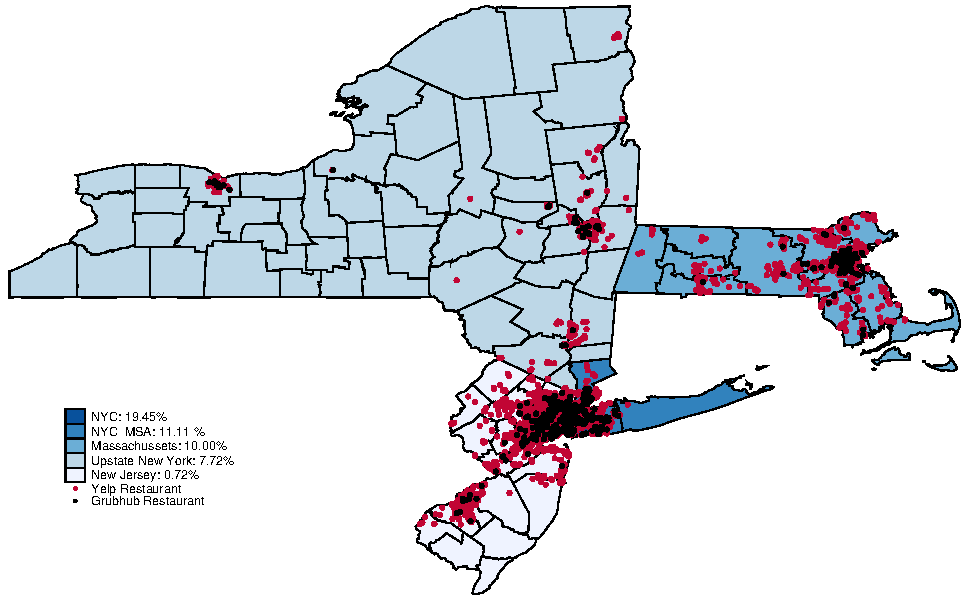
\includegraphics[scale=.75]{map_yelp.pdf}
\caption[Short Heading]{
Counties are coded by average minimum wage increase, with darker colors representing higher increases in minimum wage. The average minimum wage increase is used in New York since there are multiple levels of increases seen within a single county. Each point represents a restaurant in the sample that has menu price and item information provided on Yelp, that has been linked to the ReferenceUSA dataset and that is observed in all waves of data collection.
}
\end{figure}

\begin{figure}
\centering
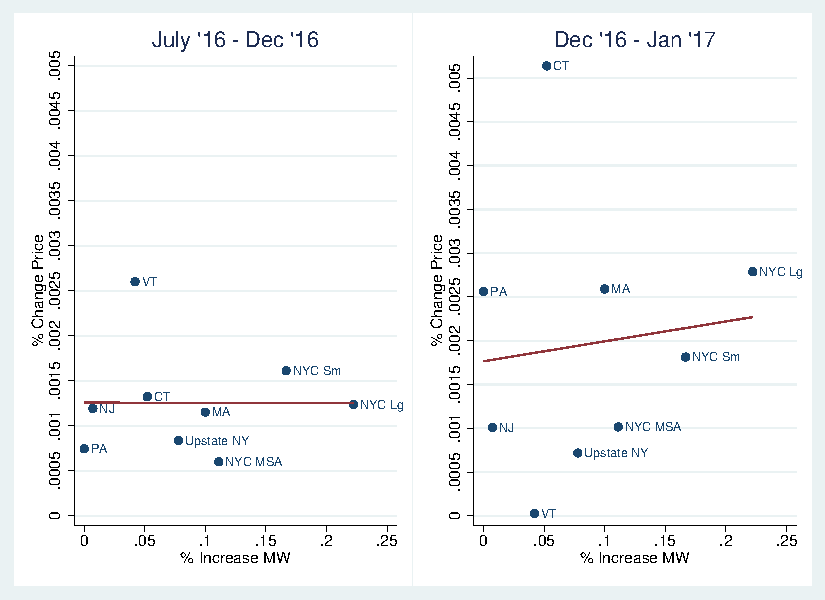
\includegraphics[scale=1]{yelp_scatter_lfit.pdf}
\caption[Short Heading]{
Percent change in price is averaged over all items for each minimum wage group. From July 2016 to December 2016 there were no changes in minimum wage laws, thus the percent increase in minimum wage reported on the x-axis is the change these restaurants would face in January of 2017. Fast food restaurants are excluded in this figure as they are in the analysis. Connecticut and Vermont both have relatively small sample sizes in the data, and so a small number of outliers in the group can heavily influence the average. In Philadelphia, PA there was a per ounce tax implemented on all soda sales and could be a mechanism of the large change in price for that group seen from December to January. 
}
\end{figure}

\begin{figure}
\centering
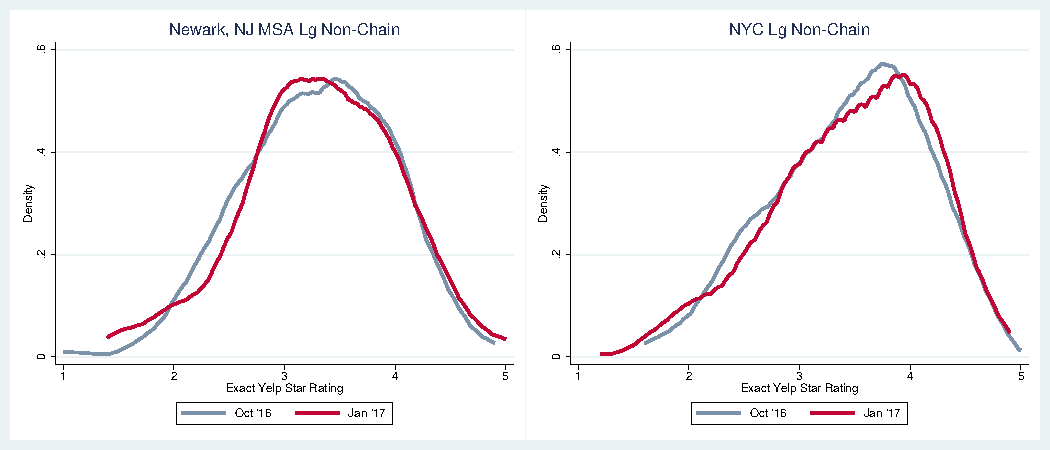
\includegraphics[scale=.75]{star_dens_ny.pdf}
\caption[Short Header]{
The plot on the left depicts the distribution of exact Yelp star ratings for large, non chain restaurants in the Newark, NJ area including restaurants in the five contiguous counties to NYC (Essex, Bergen, Hudson, Union and Monmouth) in October of 2016 and in January 2017. The plot on the right depicts the same scenario for restaurants in downtown NYC. These two groups are comparable in geographic location and restaurant characteristics, however Newark restaurants observed a 0.71\% increase in minimum wage while NYC restaurants saw a 22\% increase. There is slight movement with the New Jersey restaurants, which is to be expected since over 70\% of restaurants change ratings between observations. However, the movement in the NYC group is distinctly shift in towards the right, an indication that more restaurants are receiving higher reviews after the minimum wage hike. 
}
\end{figure}

\vspace{100mm}

\clearpage

\newpage 

\section{Tables}


\begin{table}[H]
\centering
\begin{tabularx}{1\textwidth}{ c c *{7}{Y} } \\ \hline \hline
%\begin{tabular}{ cccccc } \\ \hline \hline
& & \multicolumn{3}{c}{Regular Minimum Wage} & \multicolumn{3}{c}{Tipped Minimum Wage}\\
Group & Area & `16  & `17  & $\% \Delta$ & `16 & `17 &  $\% \Delta$  \\ \hline \hline
%&&& \\
1 &  NYC \& FF & \$10.50 & \$12.00 & 14.29\%& - & - & - \\
 2 & NY Upstate \& FF  & \$9.75 & \$10.75 & 10.26\% & - & -& - \\
3 & NYC \& Lg & \$9.00 & \$11.00 & 22.22\% & \$7.50 & \$7.50 & 0.00\%\\
4 & NYC \& Sm & \$9.00 & \$10.50 & 16.67 \% & \$7.50 & \$7.50 & 0.00\%\\
5 & NYC MSA & \$9.00 & \$10.00 & 11.11\% & \$7.50 & \$7.50 & 0.00\%\\
6 & NY Upstate & \$9.00 & \$9.70 & 7.78\% & \$7.50 & \$7.50  & 0.00\% \\
7 & Connecticut & \$9.60 & \$10.10 & 5.21\% & \$6.07 & \$6.38 & 5.11\% \\
8 & New Jersey &  \$8.38 & \$8.44 & 0.72\%  & \$2.13 & \$2.3 & 0.00\% \\
9 & Massachusetts & \$10.00 & \$11.00 & 10.00\% & \$3.00 & \$3.75  & 25.00\% \\
10 & Pennsylvania &  \$7.25 & \$7.25 & 0.00\% & \$2.83 & \$2.83 & 0.00\% \\
11 & Vermont &  \$9.60 & \$10.00 & 4.2\% & \$4.80 & \$5.00 & 4.2\% \\
\end{tabularx}
%\end{tabular}
\caption[Short Heading]{The regular and tipped minimum wage changes from 2016 to 2017 are reported by group. Groups 1 and 2 report minimum wage increases for fast-food restaurants in NYC and Upstate New York. Groups 3 and 4 report minimum wage increases for non-fast-food restaurants in NYC based on size of the restaurant. Groups 5 and 6 report minimum wage increases for non-fast-food restaurants in the contiguous counties surrounding NYC and upstate New York. Groups 7-11 report minimum wage increases for the five contiguous states surrounding New York. As shown, there were some changes in the tipped minimum wage, but the analysis in this paper will focus on impacts of changes in the regular minimum wage.
}
\end{table}

\begin{table}[H]
\centering
\begin{tabular}{l l l l l l } \\ \hline \hline
Sample & N Rest's &  \% LS & \% Chain & \% Small \\ \hline \hline
%&&& \\
Population (RUSA) & 98,114  & 18.40	& 12.10  & 75.72\\ \hline
%&&& \\
All Yelp  & 80,156  & - & -  & - \\
Yelp + Menus & 25,177 &   - & - & - \\  \cdashline{1-6}
%&&& \\ 
All Yelp + RUSA &  35,502 &  17.01 & 11.82 & 75.13 \\
Yelp + Menus + RUSA & 14,208 &  13.24 & 9.65 & 72.12\\ 
%&&& \\
Yelp Menus + Prices +  RUSA & 11,854  & 5.49 & 1.89 & 78.40 \\ 
%&&& \\
Eat24 Menus +  RUSA& 2,772  & 6.96 & 1.85 & 89.18 \\ \hline
%&&& \\
Grubhub Menus &14,005 & - & -  & -\\
Grubhub Menus + RUSA & 5,482  & 6.51 & 2.01 & 86.12 \\ \hline
\end{tabular}
\caption[Short Heading]{
Sample construction for one wave of the scrape is reported in this table. The first row shows the characteristics of the ReferenceUSA dataset, which is used in this paper as the population. The next two rows show the sample size of the total number of restaurants that are in the Yelp scrape and the number of these that post full menus on the Yelp site. These rows do not report LS, chain, or small percentages because they are not yet linked to the ReferenceUSA dataset. The subsequent four rows show the characteristics of Yelp restaurants once they are linked to the ReferenceUSA dataset. The final two rows report characteristics of restaurants who post menus on Grubhub. It can be seen from the table that all restaurants on Yelp are representative of the true population. However, limited service and chain restaurants are less likely to post menus on yelp and significantly less likely to post menus that contain prices. 
}
\end{table}



\begin{sidewaystable}
\centering
\begin{tabular}{ccccccccccccc } \\ \hline \hline
 Area & \%$\Delta$ MW & Source & \# Rest & \%LS & \%Chain & Employees & \# Items & Price/Item & Sales & Stars \\ \hline \hline
%&&& \\
 NYC \& FF  & 14.29&  Yelp & 25  & 100.00 & 100.00 & 12.72 & 67.64 & 7.90 & 874,320 & 2.76  \\
 &  & Grubhub  & 34 & 100.00 & 100.00 & 15.65 & 26.56 & 9.71 & 943,615 & - \\ \cdashline{3-12}
 NY Upstate \& FF  &10.26  &Yelp  & 6 & 100.00 & 100.00 & 7.83 & 77.16 & 6.65 &  445,000 & 3.4  \\
  &  & Grubhub & 13 & 100.00 & 100.00 & 16.46 & 26.15 & 10.61 & 943,615  & - \\ \cdashline{3-12}
NYC \& Lg & 22.22& Yelp & 611 & 3.93 &  6.54 & 30.55 & 74.79 & 14.02 & 241,3624 & 3.49 \\
 & & Grubhub & 406 & 4.67 & 1.48 & 30.62 & 105.17 & 10.95 & 2,585,000 & - \\ \cdashline{3-12}
NYC \& Sm & 16.67 & Yelp & 2,409 & 4.69 & 0.41 & 5.45 & 93.54 & 10.00 & 401,314 & 3.59 \\
& & Grubhub & 2,226 & 4.68 & 0.22 & 5.37 & 118.44 & 9.41 & 401,252 & - \\ \cdashline{3-12}
NYC MSA & 11.11 & Yelp & 425 & 7.29 & 1.17 & 10.34 & 100.68 & 11.17 & 733,378 & 3.54 \\
& & Grubhub & 341 & 6.75 & 0.89 & 6.07 & 142.79 & 9.92 & 351,557 & - \\ \cdashline{3-12}
NY Upstate & 7.78 & Yelp & 378 & 6.35 & 0.53 & 10.71 & 77.73 & 9.69 & 526,693 & 3.56  \\
& & Grubhub & 207 & 6.28 & 2.89 & 9.68 & 113.14 & 8.19 & 472,855 & - \\ \cdashline{3-12}
Connecticut & 5.21 & Yelp & 57 & 1.75 & 0.00 & 14.37 & 78.30 & 11.34 & 1,033,830 & 3.61 \\
&& Grubhub & 92 & 8.67 & 1.09 & 5.46 & 136.38 & 9.13 & 336,054 & - \\ \cdashline{3-12}
New Jersey & 0.72 & Yelp & 1,480 & 5.94 & 2.23 & 10.21 & 99.83 & 10.14 & 610,835 & 3.54 \\
& & Grubhub & 792 & 7.95 & 2.16 & 5.61 & 134.68 & 9.09& 325,266 & - \\ \cdashline{3-12}
Massachusetts & 10.00 & Yelp & 1,392 & 2.73 & 2.37 & 15.45 & 89.00 & 10.15 & 960,760 & 3.54 \\
&& Grubhub & 550 & 4.00 & 1.63 & 8.12 & 126.88 & 9.27 & 501,843 & - \\ \cdashline{3-12}
Pennsylvania & 0.00 & Yelp & 1,072 & 7.83 & 2.80 & 12.10 & 107.15 & 9.89 & 732,673 & 3.57 \\
&& Grubhub & 647 & 7.10 & 2.16 & 6.74  & 141.38 & 8.44 & 392,592 & - \\ \cdashline{3-12}
Vermont & 4.2 & Yelp & 50 & 0.00 & 0.00 & 17.08 & 85.56 & 8.94 & 701,900 & 3.54 \\
&& Grubhub & 2 & 0.00 & 0.00 & 13.5 & 128.00 &  8.82 & 614,5000 & - \\  \cdashline{3-12}
\end{tabular}
\caption[Short Heading]{
Sample sizes shown here are the number of restaurants that post full menus on Yelp or Grubhub with prices and that have been linked to the ReferenceUSA dataset. There are a larger number of total restaurants and Eat24 restaurants in the larger cities, which is to be expected given the nature of the scrape and of the delivery service. Some restaurants have menus on one website and not the other, so although there are restaurants that are in both the Grubhub and Yelp datasets, it is not to be expected that the summary statistis would be identical within groups across data sources.
}
\end{sidewaystable}


%
%\begin{table}
%\centering
%\begin{tabular}{l c c c } \\ \hline \hline
%Variable & All & LS & FS \\ \hline \hline
%&&& \\
%Percent increases & 3.02 & 2.65 & 3.04 \\
%Percent decreases & 1.58 & 1.48 & 1.59 \\
%Observations & 1,578,367 & 74,236 & 1,501,969 \\
% &&& \\
% Mean price change $|$ Increase & 25.88 & 30.74 & 25.67 \\
% Mean price change $|$ Decrease & 41.32 & 47.29 & 41.04 \\
% \end{tabular}
% \caption[Short Heading]{
%The first two rows report the share of price changes, and the observations are at the item level. The last two rows report magnitudes of increases (decreases) conditional on increase (decrease) in the price of the item.
% }
% \end{table}

\begin{table}
\centering
{
\def\sym#1{\ifmmode^{#1}\else\(^{#1}\)\fi}
\begin{tabular}{l*{8}{c}}
\hline\hline
&\multicolumn{4}{c}{Yelp}&\multicolumn{1}{c}{Eat24} &\multicolumn{3}{c}{Grubhub} \\
                    &\multicolumn{1}{c}{(1)}&\multicolumn{1}{c}{(2)}&\multicolumn{1}{c}{(3)}&\multicolumn{1}{c}{(4)}&\multicolumn{1}{c}{(5)}&\multicolumn{1}{c}{(6)}&\multicolumn{1}{c}{(7)}&\multicolumn{1}{c}{(8)}\\
                  %  &\multicolumn{1}{c}{ch\_av\_p}&\multicolumn{1}{c}{ch\_av\_p}&\multicolumn{1}{c}{ch\_av\_p}&\multicolumn{1}{c}{ch\_av\_p}&\multicolumn{1}{c}{ch\_av\_p}\\
\hline
$\Delta Ln(mw_{kt}) $&      0.0201\sym{*}  &      0.0264\sym{**} &      0.0264\sym{**} &      0.0264\sym{*}  &      0.0411      &      0.0116     &      0.0224         &      0.0270      \\
                    &   (0.00934)         &    (0.0102)         &    (0.0102)         &    (0.0107)         &    (0.0276)      &    (0.0215)         &    (0.0330)         &    (0.0363)        \\
[1em]
Chain               &                     &                     &     -0.0204\sym{**} &                     &                     &                     &                     &    -0.00578    \\
                    &                     &                     &   (0.00645)         &                     &                       &                     &                     &    (0.0221)    \\
[1em]
Employees           &                     &                     &  -0.0000270         &                     &                     &                     &                     &   -0.000384  \\
                    &                     &                     & (0.0000508)         &                     &                      &                     &                     &  (0.000205)        \\
[1em]
Sales               &                     &                     &   -3.27e-10         &                     &                     &                     &                     &    3.75e-09  \\
                    &                     &                     &  (5.78e-10)         &                     &                      &                     &                     &  (2.06e-09)   \\
[1em]
LS                  &                     &                     &    -0.00163         &                     &                     &                     &                     &    -0.00766    \\
                    &                     &                     &   (0.00280)         &                     &                      &                     &                     &   (0.00719)  \\
\hline
Group FE        &       No         &       Yes         &       Yes         &       No         &        No         & No & Yes & Yes\\
Rest. FE        &       No         &       No         &       No         &       Yes         &        Yes        & No & No & No\\
Observations        &       23502         &       23502         &       23502         &       23502         &        5051       &        5366         &        5364         &        5364        \\
\hline\hline
\multicolumn{6}{l}{\footnotesize Standard errors in parentheses}\\
\multicolumn{6}{l}{\footnotesize \sym{*} \(p<0.05\), \sym{**} \(p<0.01\), \sym{***} \(p<0.001\)}\\
\end{tabular}
}

\caption[Short Heading]{
The outcome variable for all columns is the log change in price at the restaurant level. Columns 1-4 report estimates using the full Yelp dataset. Column 5 includes only those Yelp restaurants who employ the Eat24 delivery service. Columns 6-5 report estimates using the Grubhub restaurants. Restaurant level fixed effects are not used in the Grubhub data since items are location specific and there is only one change observed, making the Grubhub dataset cross sectional. 
}
\end{table}
%
%\begin{table}
%\centering
%{
\def\sym#1{\ifmmode^{#1}\else\(^{#1}\)\fi}
\begin{tabular}{l*{3}{c}}
\hline\hline
                    &\multicolumn{1}{c}{(1)}&\multicolumn{1}{c}{(2)}&\multicolumn{1}{c}{(3)}\\
                    &\multicolumn{1}{c}{ch\_av\_p}&\multicolumn{1}{c}{ch\_av\_p}&\multicolumn{1}{c}{ch\_av\_p}\\
\hline
$ \Delta Ln(mw\_{kt}) $&      0.0116         &      0.0224         &      0.0270         \\
                    &    (0.0215)         &    (0.0330)         &    (0.0363)         \\
[1em]
chain               &                     &                     &    -0.00578         \\
                    &                     &                     &    (0.0221)         \\
[1em]
Employees           &                     &                     &   -0.000384         \\
                    &                     &                     &  (0.000205)         \\
[1em]
Sales               &                     &                     &    3.75e-09         \\
                    &                     &                     &  (2.06e-09)         \\
[1em]
LS                  &                     &                     &    -0.00766         \\
                    &                     &                     &   (0.00719)         \\
\hline
Observations        &        5366         &        5364         &        5364         \\
\hline\hline
\multicolumn{4}{l}{\footnotesize Standard errors in parentheses}\\
\multicolumn{4}{l}{\footnotesize \sym{*} \(p<0.05\), \sym{**} \(p<0.01\), \sym{***} \(p<0.001\)}\\
\end{tabular}
}

%\caption[Short Heading]{
%Grubhub rest level
%}
%\end{table}



\begin{table}
\centering
{
\def\sym#1{\ifmmode^{#1}\else\(^{#1}\)\fi}
\begin{tabular}{l*{5}{c}}
\hline\hline
                    &\multicolumn{1}{c}{(1)}&\multicolumn{1}{c}{(2)}&\multicolumn{1}{c}{(3)}&\multicolumn{1}{c}{(4)}&\multicolumn{1}{c}{(5)}\\
                    &\multicolumn{1}{c}{$ <=2.5 $}&\multicolumn{1}{c}{$ 3 $}&\multicolumn{1}{c}{$3.5$}&\multicolumn{1}{c}{ $ 4 $}&\multicolumn{1}{c}{ $  >=4.5 $ }\\
\hline
$\Delta Ln(mw\_{kt}) $&      0.0166         &      0.0669\sym{*}  &      0.0117         &      0.0207         &      0.0296         \\
                    &    (0.0454)         &    (0.0277)         &    (0.0164)         &    (0.0175)         &    (0.0271)         \\
[1em]
Chain               &     -0.0158         &     -0.0312\sym{**} &    -0.00965         &      0.0133         &           0         \\
                    &    (0.0204)         &    (0.0114)         &    (0.0118)         &    (0.0258)         &         (.)         \\
[1em]
Employees           &  -0.0000995         &   0.0000134         &   0.0000187         &  -0.0000944         &   -0.000175         \\
                    &  (0.000302)         &  (0.000123)         & (0.0000868)         & (0.0000834)         &  (0.000300)         \\
[1em]
Sales               &    8.38e-10         &   -1.20e-09         &   -7.07e-10         &   -5.61e-12         &    7.76e-10         \\
                    &  (3.28e-09)         &  (1.74e-09)         &  (1.03e-09)         &  (8.03e-10)         &  (3.16e-09)         \\
[1em]
LS                  &    -0.00137         &    -0.00716         &   -0.000726         &   -0.000238         &     0.00254         \\
                    &   (0.00982)         &   (0.00782)         &   (0.00486)         &   (0.00546)         &   (0.00572)         \\
\hline
Group FE        &        Yes         &        Yes        &        Yes         &        Yes         &        Yes         \\

Observations        &        1878         &        4014         &        7647         &        7437         &        2526         \\
\hline\hline
\multicolumn{6}{l}{\footnotesize Standard errors in parentheses}\\
\multicolumn{6}{l}{\footnotesize \sym{*} \(p<0.05\), \sym{**} \(p<0.01\), \sym{***} \(p<0.001\)}\\
\end{tabular}
}

\caption[Short Heading]{
The outcome variable for all columns is the log change in price at the restaurant level using the Yelp dataset. The restaurants are split up into subsamples by the Yelp star rating they had in April of 2016. This star rating is the exact rating rounded to the nearest half star, which is what the customers see. Group fixed effects are used for each subsample.
}
\end{table}


\begin{table}
\centering
{
\def\sym#1{\ifmmode^{#1}\else\(^{#1}\)\fi}
\begin{tabular}{l*{7}{c}}
\hline\hline
                    &\multicolumn{1}{c}{(1)}&\multicolumn{1}{c}{(2)}&\multicolumn{1}{c}{(3)}&\multicolumn{1}{c}{(4)}&\multicolumn{1}{c}{(5)}&\multicolumn{1}{c}{(6)}&\multicolumn{1}{c}{(7)}\\
                    &\multicolumn{1}{c}{All}&\multicolumn{1}{c}{Popular}&\multicolumn{1}{c}{Side}&\multicolumn{1}{c}{Sandwich}&\multicolumn{1}{c}{Entre}&\multicolumn{1}{c}{Desert}&\multicolumn{1}{c}{Other}\\
\hline
$ \Delta Ln(mw\_{kt}) $&      0.0330         &     -0.0312         &       0.156\sym{*}  &      0.0706         &      0.0542         &     -0.0289         &     -0.0682         \\
                    &    (0.0276)         &    (0.0423)         &    (0.0657)         &    (0.0466)         &    (0.0490)         &    (0.0197)         &    (0.0595)         \\
\hline
Grop FE        &      Yes         &       Yes         &       Yes         &      Yes         &      Yes         &       Yes         &      Yes         \\

Observations        &      734528         &       54986         &       85304         &      100672         &      127938         &       17409         &      165566         \\
\hline\hline
\multicolumn{8}{l}{\footnotesize Standard errors in parentheses}\\
\multicolumn{8}{l}{\footnotesize \sym{*} \(p<0.05\), \sym{**} \(p<0.01\), \sym{***} \(p<0.001\)}\\
\end{tabular}
}

\caption[Short Heading]{
The outcome variable for all columns is the log change in price at the item level using the Grubhub dataset. All regressions include group fixed effects, and errors are clustered at the restaurant level. 
}
\end{table}

\begin{table}
\centering
{
\def\sym#1{\ifmmode^{#1}\else\(^{#1}\)\fi}
\begin{tabular}{l*{3}{c}}
\hline\hline
                    &\multicolumn{1}{c}{(1)}&\multicolumn{1}{c}{(2)}&\multicolumn{1}{c}{(3)}\\
%                    &\multicolumn{1}{c}{ch\_lns}&\multicolumn{1}{c}{ch\_lns}&\multicolumn{1}{c}{ch\_lns}\\
\hline
$\Delta Ln(mw_{kt}) $&      0.0316\sym{*}  &      0.0356\sym{*}  &      0.0354\sym{*}  \\
                    &    (0.0140)         &    (0.0152)         &    (0.0152)         \\
[1em]
$\Delta Ln(p_{jkt}) $     &                     &                     &    -0.00877         \\
                    &                     &                     &   (0.00982)         \\
[1em]
Stars\_April         &                     &                     &    -0.00877\sym{***}\\
                    &                     &                     &   (0.00172)         \\
[1em]
Chain               &                     &                     &    -0.00676         \\
                    &                     &                     &   (0.00924)         \\
[1em]
Sales               &                     &                     &   -7.27e-11         \\
                    &                     &                     &  (8.23e-10)         \\
[1em]
Employees           &                     &                     &  0.00000362         \\
                    &                     &                     & (0.0000730)         \\
\hline
Group FE        &       No         &       Yes         &       Yes         \\
Observations        &       20165         &       20165         &       20156         \\
\hline\hline
\multicolumn{4}{l}{\footnotesize Standard errors in parentheses}\\
\multicolumn{4}{l}{\footnotesize \sym{*} \(p<0.05\), \sym{**} \(p<0.01\), \sym{***} \(p<0.001\)}\\
\end{tabular}
}

\caption[Short Heading]{
The outcome variable for all columns is the log change in exact Yelp star rating. The first column does not include any fixed effects or control variables. Columns 2 and 3 include minimum wage group fixed effects. Stars in April is the rounded Yelp star rating that a restaurant had prior to the minimum wage increase.
}
\end{table}


\begin{table}
\centering
\begin{tabularx}{1\textwidth}{ c c *{7}{Y} } \\ \hline \hline
& \multicolumn{6}{c}{Rounded Star Rating (S)} \\
& $<$2.5 & 2.5 & 3.0 & 3.5 & 4.0  & 4.5 & 5.0 \\ \hline \hline
$Pr(S)|\Delta ln(mw)=0.00$ & 0.0468 & 0.0957  & 0.1869 & 0.2612 & 0.2643 & 0.1298 & 0.0152 \\
$Pr(S)|\Delta ln(mw)=0.10$ & 0.0462 & 0.0949 & 0.1860 & 0.2610 & 0.2654 & 0.1312 & 0.0154 \\ \hline
\% Change & -0.85 & -0.84 & -0.48 & 0.10 & 0.42 & 1.00 & 1.32 \\ \hline \hline
\end{tabularx}
\caption[Short Heading]{
This table reports post estimation probabilities from the ordered probit model. The first column shows predicted probabilities of having the given star rating conditional on no increase in minimum wage. The second column shows predicted probabilities of having the given star rating conditional on a 10\% increase in minimum wage. For these calculations, LS and chain are set at zero and sales and employees are set at the sample mean. 
}
\end{table}

\begin{table}
\centering
{
\def\sym#1{\ifmmode^{#1}\else\(^{#1}\)\fi}
\begin{tabular}{l*{3}{c}}
\hline\hline
                    &\multicolumn{1}{c}{(1)}&\multicolumn{1}{c}{(2)}&\multicolumn{1}{c}{(3)}\\
                    &\multicolumn{1}{c}{Total Items}&\multicolumn{1}{c}{Hours}&\multicolumn{1}{c}{Days}\\
\hline
$\Delta Ln(mw_{kt}) $&      0.0757         &      -0.477         &     -0.0215         \\
                    &     (3.453)         &     (0.646)         &    (0.0212)         \\
[1em]
Chain               &       3.332         &      0.0643         &      0.0106         \\
                    &     (2.193)         &     (0.387)         &    (0.0127)         \\
[1em]
Employees           &     0.00874         &     0.00326         &   -0.000128         \\
                    &    (0.0173)         &   (0.00314)         &  (0.000103)         \\
[1em]
Sales               &    8.08e-08         &   -3.49e-08         &   -5.73e-10         \\
                    &(0.000000196)         &  (3.51e-08)         &  (1.15e-09)         \\
[1em]
LS                  &       0.615         &       0.226         &    0.000880         \\
                    &     (0.953)         &     (0.190)         &   (0.00624)         \\
\hline
Group FE        &       Yes         &       Yes         &       Yes         \\
Observations        &       23511         &       19356         &       19356         \\
\hline\hline
\multicolumn{4}{l}{\footnotesize Standard errors in parentheses}\\
\multicolumn{4}{l}{\footnotesize \sym{*} \(p<0.05\), \sym{**} \(p<0.01\), \sym{***} \(p<0.001\)}\\
\end{tabular}
}

\caption[Short Heading]{
The outcome variable for column 1 is the change in total items per restaurant. The outcome variable for column 2 is the change in total hours open per week, and the the outcome variable for column 3 is the change in total number of days open per week. Although imprecisely estimated, the point estimates show that restaurants are not significantly changing the number of menu items offered, but columns 2 and 3 indicate that restaurants may be cutting back on hours of operation.
}
\end{table}

%\begin{table}
%\centering
%{
\def\sym#1{\ifmmode^{#1}\else\(^{#1}\)\fi}
\begin{tabular}{l*{4}{c}}
\hline\hline
                    &\multicolumn{1}{c}{(1)}&\multicolumn{1}{c}{(2)}&\multicolumn{1}{c}{(3)}&\multicolumn{1}{c}{(4)}\\
                    &\multicolumn{1}{c}{ch\_av\_p}&\multicolumn{1}{c}{ch\_av\_p}&\multicolumn{1}{c}{ch\_av\_p}&\multicolumn{1}{c}{ch\_av\_p}\\
\hline
$\Delta Ln(MW\_{kt}) $&      0.0248         &      0.0387         &      0.0387         &      0.0264\sym{*}  \\
                    &    (0.0258)         &    (0.0277)         &    (0.0277)         &    (0.0107)         \\
[1em]
Chain               &                     &                     &    -0.00266         &                     \\
                    &                     &                     &    (0.0668)         &                     \\
[1em]
Employees           &                     &                     &   0.0000384         &                     \\
                    &                     &                     &  (0.000274)         &                     \\
[1em]
Sales               &                     &                     &   -2.84e-09         &                     \\
                    &                     &                     &  (2.53e-09)         &                     \\
\hline
Observations        &        4173         &        4173         &        4173         &       23502         \\
\hline\hline
\multicolumn{5}{l}{\footnotesize Standard errors in parentheses}\\
\multicolumn{5}{l}{\footnotesize \sym{*} \(p<0.05\), \sym{**} \(p<0.01\), \sym{***} \(p<0.001\)}\\
\end{tabular}
}

%\caption[Short Heading]{
%yelp w/ only gh 
%}
%\end{table}

\end{document}
